\documentclass[11pt]{article}

\usepackage[margin=1in, headheight=14.5pt]{geometry}
\usepackage{amsfonts, amsmath, amssymb}
\usepackage{enumitem}
\usepackage[none]{hyphenat}
\usepackage{fancyhdr}
\usepackage[spanish, es-noshorthands]{babel}
\usepackage[spanish, calc]{datetime2}
\usepackage{fmtcount}
\usepackage{graphicx}
\usepackage{float}
\usepackage[nottoc, notlot, notlof]{tocbibind}
\usepackage{tocloft}
\usepackage[utf8]{inputenc}
\usepackage{parskip}
\usepackage{xcolor}
\usepackage{cancel}
\usepackage{textcomp}
\usepackage{pgfplots}
\usepackage{tikz}
\usetikzlibrary{shapes.misc}
\usepackage{polynom}
\usetikzlibrary{datavisualization}
\usetikzlibrary{datavisualization.formats.functions}
\pgfplotsset{compat=1.15}
\usepackage{mathrsfs}
\usetikzlibrary{arrows}
\usepackage{adjustbox}

\newcommand{\dropsign}[1]{\smash{\llap{\raisebox{-.5\normalbaselineskip}{$#1$\hspace{2\arraycolsep}}}}}%


\parindent 0ex

\pgfplotsset{width=10cm,compat=1.9}

\def\imj{\mathrm{j}}
\def\sen{\mathrm{sen}}

\newcommand{\lapl}[1]{\mathscr{L} \left\lbrace {#1} \right\rbrace}
\newcommand{\ilapl}[1]{\mathscr{L}^{-1} \left\lbrace {#1} \right\rbrace}

\renewcommand\cftsecleader{\cftdotfill{\cftdotsep}}
\renewcommand{\baselinestretch}{1.1}
\newcommand*\circled[1]{\tikz[baseline=(char.base)]{
		\node[shape=circle,draw,inner sep=2pt] (char) {#1};}}
	
\newcommand{\highlight}[2]{\colorbox{#1}{$\displaystyle #2$}}

\graphicspath{{\ProjectRoot/commons/img/}}

\newcommand*{\ProjectRoot}{../../matematica-superior}


\begin{document}
		
	\begin{titlepage}
		\begin{center}
			\vspace*{0.5cm}
			\Large{\textbf{Universidad Tecnológica Nacional}}\\
			\Large{\textbf{Facultad Regional Buenos Aires}}\\
			\begin{center}
				
\includegraphics[scale=0.4]{logoutn.png}
			\end{center}
			\vfill
			\line(1,0){400}\\
			\vspace*{0.3cm}
			\huge{\textbf{Matemática Superior}}\\
			\Large{\textbf{Unidad 10: Diferenciación e Integración numérica}}\\
			\textit{\large{(incluye Polinomios de Legendre)}} \\
			\large{Ejercicios resueltos}
			\line(1,0){400}\\
			\vfill
			Tomás Moreira \\
			
			\DTMnewdatestyle{mydate}{%
				\renewcommand{\DTMdisplaydate}[4]{%
					\DTMMonthname{##2} \number##1
				}
				\renewcommand{\DTMDisplaydate}{\DTMdisplaydate}
			}
			
			\DTMsetdatestyle{mydate}
			\today
				
				
		\end{center}
	\end{titlepage}

	\tableofcontents
	\thispagestyle{empty}
	\clearpage

	\setcounter{page}{1}
	
	\section{Práctica Polinomios de Legendre}
	\subsubsection{Ejercicio 32}
	Dadas las siguientes funciones continuas, aproxime por un polinomio de Mínimos cuadrados en los intervalos indicados y grafique.
	
	Los polinomios de Legendre son polinomios ortogonales en el intervalo $[-1;1]$ que se pueden usar para aproximar funciones.
	
	\begin{itemize}
		\item Con ellos, evitamos resolver sistemas de ecuaciones, que con muchas variables pueden ser difíciles de resolver
		\item El resultado es el mismo usando los polinomios de Legendre que resolviendo el sistema de ecuaciones
		\item Para resolver grados sucesivos me sirven los cálculos anteriores. Es decir, si calculé $a_0$ y $a_1$ para una recta, estos mismos valores me sirven para luego calcular el polinomio de grado 2.
		\item A veces las integrales de Legendre pueden resultar complicadas.
		\item Estamos restringidos a trabajar en el intervalo [-1;1]
	\end{itemize}

	Nosotros vamos a usar polinomios de Legendre HASTA de grado 2.
	
	Para aproximar por Legendre, debemos tener en cuenta la fórmula:
	
	$P_n(x)=a_0 \varphi_0(x)+a_1 \varphi_1(x)+a_2 \varphi_2(x)+\dots a_n\varphi_n(x)$
	
	Donde $\displaystyle a_n=\frac{1}{\left\lVert \varphi_n(x) \right\rVert}\int_{-1}^{1}f(x)\varphi_n(x)$
	
	Los primeros polinomios de Legendre, y sus normas son:
	
	$\displaystyle \varphi_0(x)=1, \;\;\;\; \left\lVert\varphi_0(x) \right\rVert=2$
	
	$\displaystyle \varphi_1(x)=x, \;\;\;\; \left\lVert\varphi_1(x) \right\rVert=\frac{2}{3}$
	
	$\displaystyle \varphi_2(x)=\frac{1}{2}(3x^2-1), \;\;\;\; \left\lVert\varphi_2(x) \right\rVert=\frac{2}{5}$
	
	En forma genérica:
	
	$\displaystyle \left\lVert\varphi_k(x) \right\rVert=\frac{2}{2k+1}$\\
	
	\begin{itemize}
		\item[e)] $f(x)=x^2e^x$ en $[-1;1]$ por una recta.
	\end{itemize}

	Para usar los polinomios de Legendre, primero hay que fijarse el intervalo de trabajo. En este caso coincide el intervalo de la función con el necesario para Legendre.
	
	Segundo, tenemos que calcular los $a_n$. Como estamos en el caso de la recta, debemos calcular $a_0$ y $a_1$, para usarlos en:
	
	$P_1(x)=a_0\varphi_0(x)+a_1\varphi_1(x)$
	
	$\displaystyle a_0=\frac{1}{\lVert \varphi_0(x) \rVert} \int_{-1}^{1}x^2e^x\cdot \varphi_0(x)=\frac{1}{2} \int_{-1}^{1}x^2e^x\cdot 1=0.439442$
	
	$\displaystyle a_1=\frac{1}{\lVert \varphi_1(x) \rVert} \int_{-1}^{1}x^2e^x\cdot \varphi_1(x)=\frac{3}{2} \int_{-1}^{1}x^2e^x\cdot x=0.674261$
	
	Con estos valores, armamos el polinomio de Legendre:
	
	$P_1(x)=0.439442\cdot1+0.674261\cdot x$
	
	\textit{está mal la respuesta de la guía}\\

	\begin{itemize}
		\item[f)] $f(x)=(2x)^3$ en $[0;1]$ por una recta y por una parábola.
	\end{itemize}

	De nuevo, primero, ver el intervalo. En este caso no coinciden!! Entonces...¿se puede resolver el ejercicio?
	
	Si, hay que hacer un cambio de variable. $[0;1]\rightarrow[-1;1]$
	
	Usamos $\displaystyle x=\frac{a+b}{2}+\frac{b-a}{2}t \implies x=\frac{1}{2}+\frac{1}{2}t=\frac{t+1}{2} \implies t=2x-1$
	
	Y ahora si, nuestra función está en el $[-1;1]$. Primero, reemplazamos el cambio de variable:
	
	$\displaystyle f(t)=\left(2\left(\frac{t+1}{2}\right)\right)^3=(t+1)^3$
	
	Calculemos la recta:
	
	$\displaystyle a_0=\frac{1}{2}\int_{-1}^{1}(t+1)^3dt=2$
	
	$\displaystyle a_1=\frac{3}{2}\int_{-1}^{1}(t+1)^3\cdot t dt=2=3.6$
	
	\textbf{Importante:} al polinomio de Legendre dentro de la integral no hay que aplicarle la formula del cambio de variable!!! (ya es ortogonal en el -1 a 1)
	
	$P_1(t)=2+3.6t \implies P_1(x)=2+3.6(2x-1)=2+7.2x-3.6 \implies P_1(x)=7.2x-1.6$
	
	Ahora, para la parábola solo hay que calcular el $a_2$:
	
	$P_2(x)=a_0\varphi_0(x)+a_1\varphi_1(x)+a_2\varphi_2(x)=7.2x-1.6+a_2\varphi_2(x)$
	
	$\displaystyle a_2=\frac{5}{2}\int_{-1}^{1}(t+1)^3\frac{1}{2}(3t^2-1)=2$
	
	$\displaystyle a_2 \varphi_2(t)=2\cdot \frac{1}{2}(3t^2-1)$
	
	$a_2 \varphi_2(x)=3\left(2x-1\right)^2-1=3(4x^2-4x+1)-1=12x^2-12x+2$
	
	$P_2(x)=7.2x-1.6+12x^2-12x+1\implies P_2(x)=12x^2-4.8x+0.4$
	
	\section{Ejercicio 1}
	Dada la siguiente tabla de datos:\\
	\begin{tabular}{|c|c|c|c|}
		\hline
		i & 0 & 1 & 2\\
		\hline
		$x_i$ & 0.349 & 0.436 & 0.523 \\
		\hline
		$y_i$ & 0.34202 & 0.42262 & 0.5 \\
		\hline
	\end{tabular}

	\begin{enumerate}[label=\alph*)]
		\item Estime la primer derivada de la función $f(x)$ en $x=0.436$ utilizando las diferencias progresivas, regresivas y centrales.
		\item Estime la segunda derivada en $x=0.436$
	\end{enumerate}

	\textbf{Para el inciso a)}\\
	Primero, recordemos	que necesitamos una función tabulada, y luego, tener en cuenta que\\ $h=x_{i+1}-x_i$, siendo $h$ la distancia del intervalo entre cada valor de la tabla, también llamado tamaño de paso.
	
	Debemos recordar las fórmulas para primer derivada:
	
	$\displaystyle f'(x_i)\approxeq \frac{f(x_{i+1})-f(x_i)}{h} \rightarrow$ 1° diferencia progresiva
	
	$\displaystyle f'(x_i)\approxeq \frac{f(x_{i})-f(x_{i-1})}{h} \rightarrow$ 1° diferencia regresiva
	
	$\displaystyle f'(x_i)\approxeq \frac{f(x_{i+1})-f(x_{i-1})}{2h} \rightarrow$ 1° diferencia central
	
	Por ende, para nuestro caso:
	
	$h=0.087$
	
	$\displaystyle f'(0.436)_{\text{prog}}=\frac{0.5-0.42262}{0.087}=0.889425$
	
	$\displaystyle f'(0.436)_{\text{regr}}=\frac{0.42262-0.34202}{0.087}=0.926437$
	
	$\displaystyle f'(0.436)_{\text{ctrl}}=\frac{0.5-0.34202}{2\cdot 0.087}=0.907931$
	
	\textbf{Para el inciso b):}
	
	Recordemos ahora las fórmulas para la segunda diferencia:
	
	$\displaystyle f''(x_i)=\frac{f(x_{i+2})-2f(x_{i+1})+f(x_i)}{h^2}\rightarrow$ 2° diferencia progresiva
	
	$\displaystyle f''(x_i)=\frac{f(x_{i})-2f(x_{i-1})+f(x_{i-2})}{h^2}\rightarrow$ 2° diferencia regresiva
	
	$\displaystyle f''(x_i)=\frac{f(x_{i+1})-2f(x_{i})+f(x_{i-1})}{h^2}\rightarrow$ 2° diferencia central
	
	En nuestro caso solo podemos con la fórmula central, ya que nos falta un valor siguiente en la progresiva, y un valor anterior en la regresiva:
	
	$\displaystyle f''(0.436)=\frac{0.5-2\cdot 0.42262 + 0.34202}{(0.087)^2}=-0.425419$
	
	\section{Ejercicio 2}
	Aproxime $f'(150)$ y $f''(180)$ para la función $f(x)$ dada en la tabla \\
	\begin{tabular}{|c|c|c|c|c|c|c|}
		\hline
		i & 0 & 1 & 2 & 3 & 4 & 5 \\
		\hline
		$x_i$ & 0 & 60 & 120 & 180 & 240 & 300\\
		\hline
		$f(x_i)$ & 0 & 0.0824 & 0.2747 & 0.6502 & 1.3851 & 3.2229\\
		\hline
	\end{tabular}

	Para aproximar $f'(150)$ (que $f(150)$ es un valor que no tenemos en la tabla) la única forma de calcularlo es mediante la diferencia central:
	
	Usamos $h=30$, debido a que la distancia desde $x=150$ a 120 y 180 es 30, en este caso \textbf{\underline{no}} debemos usar $h=60$.
	
	$\displaystyle f'(150)=\frac{0.6502-0.2747}{2\cdot 30}=0.0062583$
	
	Para $f''(180)$ podemos usar cualquier fórmula. En este caso si debemos usar $h=60$ ya que vamos a usar $x_i$ y $f_i$ de la tabla.
	
	$\displaystyle f''(180)_{\text{prog}}=\frac{3.2229-2\cdot 1.3851 + 0.6502}{(60)^2}=0.000306361$
	
	$\displaystyle f''(180)_{\text{regr}}=\frac{0.6502-2\cdot 0.2747 + 0.0824}{(60)^2}=0.000050888$
	
	$\displaystyle f''(180)_{\text{ctl}}=\frac{1.3851-2\cdot 0.6502 + 0.2747}{(60)^2}=0.000099833$
	
	Comentarios finales:
	
	Siempre que se pueda, usar la fórmula central ya que es la que aproxima con más precisión. Usar las otras cuando no se pueda usar la fórmula central.
	
	
	\section{Ejercicio 4}
	Indique el valor de verdad de las siguientes proposiciones, justificando sus respuestas:
	
	\begin{enumerate}[label=\alph*)]
		\item No es posible calcular una aproximación de $f'(x_i)$ si no se conoce el valor de $f(x_i)$
		\item Si se dispone de una tabla con valores $f_0, f_1,\dots,f_n (n\ge4)$, entonces se puede calcular aproximadamente la derivada segunda de $f_2$ usando diferencias progresivas.
	\end{enumerate}

	\textbf{Inciso a:} es falso, vimos un ejemplo en el ejercicio 2, calculamos $f'$ para un valor de $x$ que no conocíamos, usando la diferencia central.
	
	\textbf{Inciso b:} es verdadero. Como es $n \ge 4$, tenemos $f_0, f_1, f_2, f_3$ y $f_4$ para calcular la diferencia progresiva, necesitamos $f_2$ y dos valores siguientes más, $f_3$ y $f_4$ en nuestro caso. Por lo tanto, es verdadero.

	\section{Ejercicio 6}
	Dada la función $f(x)=1+x^3$ en $[0,2]$ calcule la integral:
	\begin{enumerate}[label=\alph*)]
		\item en forma analítica
		\item aproximando mediante Trapecios con $h=1, h=0.5, h=0.2$
		\item aproximando mediante Simpson con $h=1$
		\item calcule los errores y extraiga conclusiones
	\end{enumerate}

	\textbf{Inciso a}
	
	$\displaystyle \int_{0}^{2}(1+x^3)dx=\left[ x+\frac{x^4}{4}\right]_0^2=6$
	
	\textbf{Inciso b}\\	
	Armamos las tablitas:
	
	\begin{tabular}{|c|c|c|}
		\hline
		$i$ & $x_i$ & $f(x_i)$ \\
		\hline
		0 & 0 & 1 \\
		\hline
		1 & 1 & 2 \\
		\hline
		2 & 2 & 9 \\
		\hline
	\end{tabular}
	\hspace{2cm}
	\begin{tabular}{|c|c|c|}
		\hline
		$i$ & $x_i$ & $f(x_i)$ \\
		\hline
		0 & 0 & 1 \\
		\hline
		1 & 0.5 & 1.125 \\
		\hline
		2 & 1 & 2 \\
		\hline
		3 & 1.5 & 4.375 \\
		\hline
		4 & 2 & 9 \\
		\hline
	\end{tabular}
	\hspace{2cm}
	\begin{tabular}{|c|c|c|}
		\hline
		$i$ & $x_i$ & $f(x_i)$ \\
		\hline
		0 & 0 & 1 \\
		\hline
		1 & 0.2 & 1.008 \\
		\hline
		2 & 0.4 & 1.064 \\
		\hline
		3 & 0.6 & 1.216 \\
		\hline
		4 & 0.8 & 1.512 \\
		\hline
		5 & 1 & 2 \\
		\hline
		6 & 1.2 & 2.728 \\
		\hline
		7 & 1.4 & 3.744 \\
		\hline
		8 & 1.6 & 5.096 \\
		\hline
		9 & 1.8 & 6.832 \\
		\hline
		10 & 2 & 9 \\
		\hline
	\end{tabular}

	Usando la fórmula de trapecios:
	
	$\displaystyle A_T=\frac{h}{2}(E+2P)$, donde $h$ es el tamaño de paso, $E$ es la suma de los extremos de la tabla, y $P$ es la suma de los otros puntos:
	
	Para $h=1$: $\displaystyle A_T=\frac{1}{2}((1+9)+2\cdot(2))=7$
	
	Para $h=0.5$: $\displaystyle A_T=\frac{0.5}{2}((1+9)+2\cdot(1.125+2+4.375))=6.25$
	
	Para $h=0.2$: $\displaystyle A_T=\frac{0.2}{2}((1+9)+2\cdot(1.008+1.064+1.216+1.512+2+2.728+3.744+5.096+6.832))=6.0392$
	
	\textbf{Inciso c}\\
	\begin{tabular}{|c|c|c|}
		\hline
		$i$ & $x_i$ & $f(x_i)$ \\
		\hline
		0 & 0 & 1 \\
		\hline
		1 & 1 & 2 \\
		\hline
		2 & 2 & 9 \\
		\hline
	\end{tabular}

	Ahora, tenemos que recordar la fórmula de Simpson:
	
	$\displaystyle A_S=\frac{h}{3}(E+4I+2P)$
	
	Donde $h$ es el tamaño de paso, $E$ es la suma de los extremos de la tabla, $I$ es la suma de las posiciones impares y $P$ la suma de las posiciones pares. Hay que aclarar que los extremos NO se usan ni en $I$ ni $P$.
	
	\textbf{IMPORTANTÍSIMO:} para poder aplicar la regla de Simpson, debemos considerar una cantidad par de subintervalos (lo que se traduce en una cantidad impar de puntos).
	
	Con $h=1$: $\displaystyle A_S=\frac{1}{3}(1+9+4\cdot 2 + 2\cdot 0)=6$
	
	\textbf{Inciso d}\\
	Como vemos, Simpson dio exacto, eso tiene que ver con la fórmula del error (más adelante lo vamos a ver). En cambio, para trapecios, a medida que achicamos el $h$, aumenta progresivamente su precisión.

	\section{Ejercicio 9}
	Halle el volumen del siguiente cuerpo (en revolución) $\displaystyle V=\int_{a}^{b}f(x)^2dx$ siendo $x^2+\frac{y^2}{9}=1$
	\begin{enumerate}[label=\alph*)]
		\item Usando Trapecios con $h=1$
		\item Usando Simpson con $h=1$
	\end{enumerate}

	El cuerpo en cuestión es una elipse:
	
	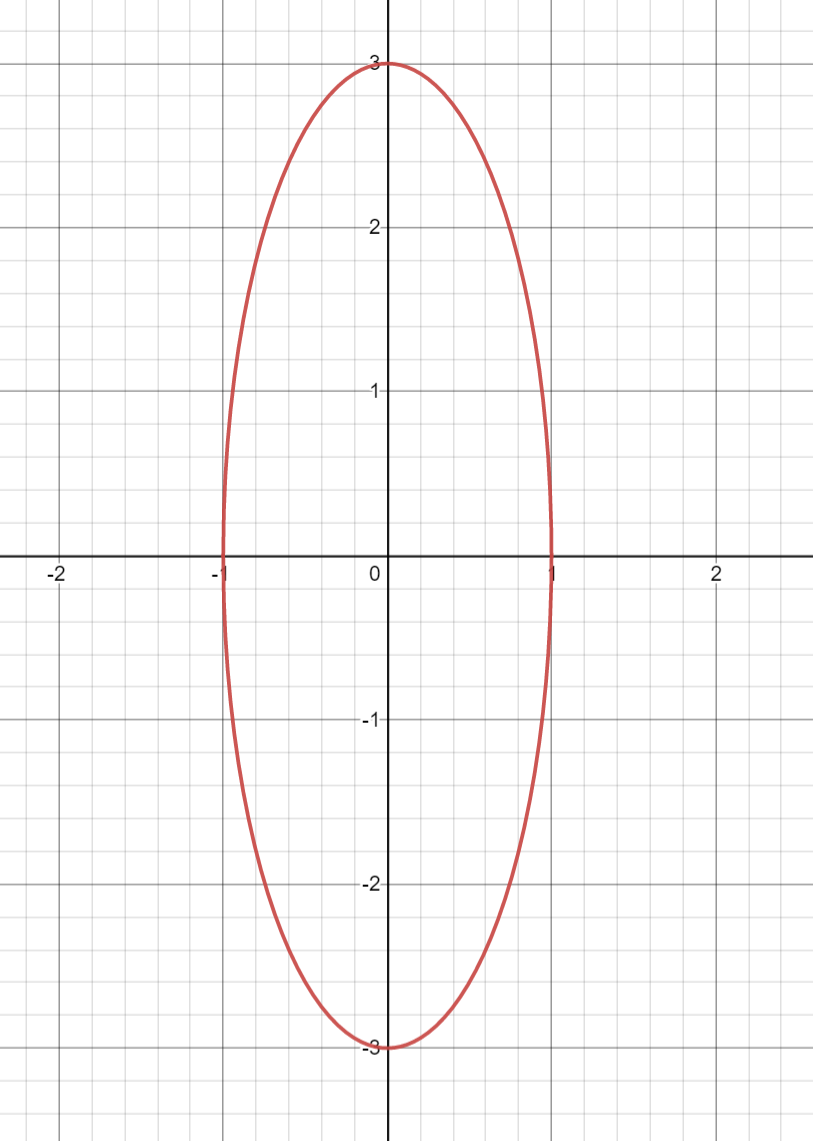
\includegraphics[scale=0.6]{10-IntegracionNumerica/9.png}
	
	Para hallar el volumen del cuerpo en revolución hay que imaginarse a la elipse girando sobre su eje.
	
	Sabemos también que $y=f(x)$, entonces dada la fórmula, vamos a despejar:
	
	$y^2=9(1-x^2)$
	
	Y listo, no hace falta aplicar cuadrado a ambos miembros, ya que necesitamos $y^2$.
	
	Los límites de la integral están dados por los valores de x de la elipse, es decir $[-1;1]$
	
	Hacemos tablita de valores:
	
	\begin{tabular}{|c|c|c|}
		\hline
		$i$ & $x_i$ & $f(x_i)$ \\
		\hline
		0 & -1 & 0 \\
		\hline
		1 & 0 & 9 \\
		\hline
		2 & 1 & 0 \\
		\hline
	\end{tabular}

	\textbf{Inciso a}
	
	Debemos usar la fórmula de Trapecios: $\displaystyle A_T=\frac{1}{2}((0+0)+2\cdot(9))=9$
	
	\textbf{Inciso b}

	Debemos usar la fórmula de Simpson: $\displaystyle A_S=\frac{1}{3}((0+0)+4\cdot(9))=12$
	
	\section{Ejercicio 14}
	Indique el valor de verdad de las siguientes proposiciones y justifique:
	
	\begin{itemize}
		\item[a)] Sea $f(x)$ una función positiva y cóncava hacia abajo en $[a,b]$, sea $A$ el valor de la integral calculada por el método de los trapecios $\displaystyle \implies A<\int_{a}^{b}f(x)dx$
	\end{itemize}
		
		Esta afirmación es \textbf{verdadera}. Para cualquier función concava hacia abajo en un intervalo, el método de trapecios aproximará por defecto:
		
		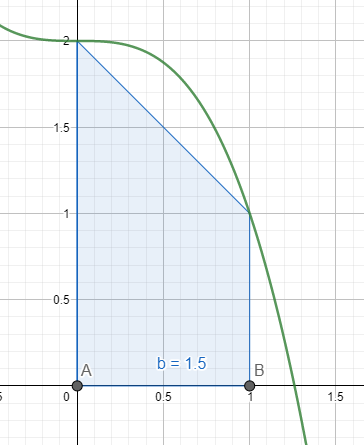
\includegraphics[scale=0.75]{10-IntegracionNumerica/14a.png}
		
		Por ende, el área real será mayor al área de trapecios.
		
		Esto tiene su teoría en la fórmula de error de trapecios:
		
		$\displaystyle e_T=-\frac{b-a}{12}\cdot h^2 \cdot f''(\xi)$ $\;\;\;\; a\le \xi \le b$
		
		Las fórmulas de error las podemos ver como $A_{\text{REAL}}=A_M+e_M$
		
		($M$ es el método con el que calculamos la integral).
		
		Luego, si la función es cóncava hacia abajo en un intervalo $(a,b)$, entonces $f''(x)<0$ en $(a,b)$, por ende el error será una cantidad positiva, lo que implica que además del área de trapecios, hay que sumarle un cachito (el error) para que sea igual al área real.
		
		El que decide el signo del error es siempre el factor de la derivada, ya que $b-a$ es siempre mayor a 0, y $h^2$ también.
		
		Si la función fuese cóncava hacia arriba en $(a,b)$, $f''(x)>0$ en $(a,b)$, el error sería una cantidad negativa, por ende, al área de trapecios hay que restarle cierto error para obtener el valor exacto.\\

	\begin{itemize}
		\item[b)] Si al calcular $\displaystyle \int_{a}^{b}f(x)dx$ por trapecios se obtiene el valor exacto $\implies f''(x)=0$ en todo $x \in (a,b)$
	\end{itemize}

	\textbf{FALSO}. Si por ejemplo, agarramos una función impar en un intervalo simétrico, el cálculo por trapecios daría 0, se compensan las áreas.
	
	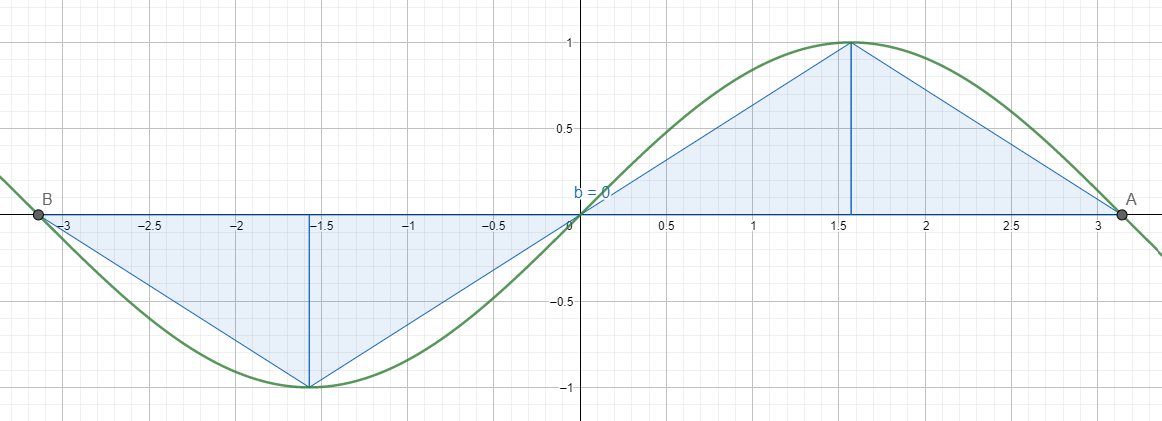
\includegraphics[scale=0.6]{10-IntegracionNumerica/14b.png}\\
	
	\begin{itemize}
		\item[c)] Si al calcular $\displaystyle \int_{a}^{b} f(x)dx$ por Simpson se obtiene error cero $\implies f(x)$ es polinómica de grado $\le 3$. 
	\end{itemize}

	Es \textbf{falso}, al igual que el ejercicio anterior, para una función impar las áreas en este caso de los polinomios interpolantes, se compensan.
		
	\begin{itemize}
		\item[d)] El error en la integración por Simpson de $f(x)=ax^3+bx^2+10$ en $(0,p)$ depende exclusivamente del valor de $p$.
	\end{itemize}

	\textbf{Falso}. Debido a que $f$ es una función polinómica de grado 3.
	
	La fórmula del error de Simpson es:
	
	$\displaystyle e_S=-\frac{b-a}{180}\cdot h^4 \cdot f^{(IV)}(\xi) \;\;\;\; a \le \xi \le b$
	
	La derivada cuarta de un polinomio de grado es 0, por ende el error es 0.\\
	
	\begin{itemize}
		\item[e)] $\forall a \in \mathbb{Z}:$ es posible resolver la integral de una función $f(x)$ en el intervalo $(a,16a)$ por el método de Simpson con $h=0.15$
	\end{itemize}

	Tenemos que verificar si esta integral tiene cantidad par de subintervalos:
	
	$\displaystyle N=\frac{b-a}{h}=\frac{16a-a}{0.15}=\frac{15a}{0.15}=100a$
	
	$100a$ es un número par $\forall a$, por ende, se puede usar el método de Simpson. \textbf{Verdadero}.\\
	
	\begin{itemize}
		\item[f)] La integral de la función $f(x)=e^{|x|}\cdot \sen(x)$ entre $-a$ y $a$ (con $a \in \mathbb{R}^+$) calculada por el método de Trapecios con una cantidad par de subintervalos da siempre exacta. 
	\end{itemize}

	Tenemos un intervalo simétrico, así que, podemos jugar con la paridad de las funciones.
	
	$e^{|x|}$ es una función par.\\
	$\sen(x)$ es una función impar.
	
	El producto de ambas da una función impar. Entonces la afirmación es \textbf{verdadera}, ya que trapecios siempre dará exacto (da siempre 0).\\
	
	\begin{itemize}
		\item[g)] Existe $h \in \mathbb{R}$ tal que $\displaystyle \int_{-1}^{1} \frac{\sen(\pi x)}{\pi x}dx$ calculada por Trapecios dé mayor que la exacta.
	\end{itemize}
	
	\textbf{Falso}. Es una función cóncava hacia abajo en $(-1,1)$, entonces trapecios aproximará por defecto (el área de trapecios será siempre menor):
	
	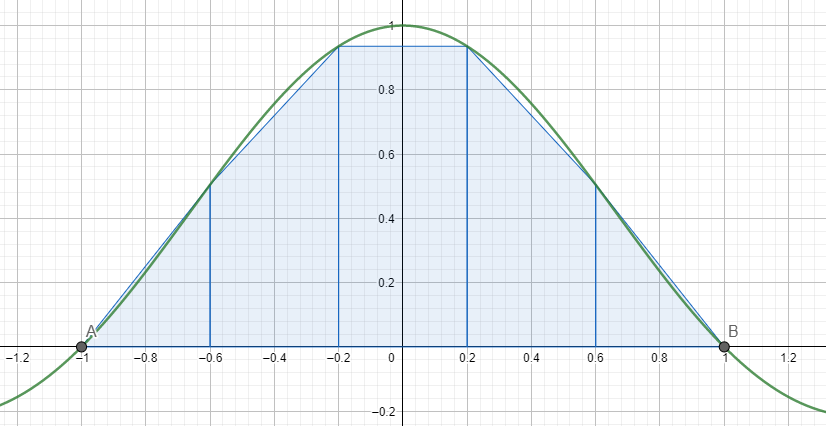
\includegraphics[scale=0.6]{10-IntegracionNumerica/14g.png}\\
	
	\begin{itemize}
		\item[h)] No es posible calcular $\displaystyle \int_{0}^{2} x^2e^xdx$ por el método de Simpson con $h=0.4$ 
	\end{itemize}

	Veamos si tiene cantidad par de subintervalos:
	
	$\displaystyle N=\frac{2-0}{0.4}=5$
	
	Tiene cantidad impar, por ende no se puede aplicar el método de Simpson, es \textbf{verdadero}.

	\section{Ejercicio 16}
	Halle el mayor valor de $h \in \mathbb{Q}$ y no periódico tal que al calcular las siguientes integrales en los intervalos dados, el error sea menor al $\varepsilon$ fijado.
	
	\begin{enumerate}
		\item[a)] $\displaystyle I=\int_{1}^{5}x^2\ln(x)dx$ por Simpson con $\varepsilon <10^{-5}$
		\item[e)] $\displaystyle I=\int_{0}^{5}(x+1)^5dx$ por Simpson con $\varepsilon < 10^{-2}$
		\item[f)] $\displaystyle I=\int_{1}^{5}x^3 \ln(x)dx$ por Trapecios con $\varepsilon<10^{-5}$
	\end{enumerate}

	\textbf{Atención, cualquier similitud con ejercicios de parcial/final es pura coincidencia}
	
	\textbf{Inciso a}
	
	Para este tipo de ejercicios debemos acotar las fórmulas de error, de la siguiente manera:
	
	$\displaystyle |e_T|=\left| \frac{b-a}{12} \right|h^2 \max_{a\le \xi \le b} \left|f''(\xi) \right|<\varepsilon$
	
	$\displaystyle |e_S|=\left| \frac{b-a}{180} \right|h^4 \max_{a\le \xi \le b}  \left|f^{(IV)}(\xi) \right|<\varepsilon$
	
	Vamos a acotar nuestra función del ejercicio, nos piden por Simpson. Así que primero, calculemos las derivadas para poder calcular el tercer factor.
	
	$\displaystyle f(x)=x^2\ln(x)$
	
	$\displaystyle f'(x)=2x\cdot \ln(x)+x^2\cdot \frac{1}{x}=2x\cdot \ln(x)+x$
	
	$\displaystyle f''(x)=2\ln(x)+2x\frac{1}{x}+1=2\ln(x)+3$
	
	$\displaystyle f'''(x)=\frac{2}{x}$
	
	$\displaystyle f^{(IV)}(x)=-\frac{2}{x^2}$
	
	Esta última expresión alcanza su máximo en el intervalo $[1,5]$ en $x=1$
	
	$\displaystyle f^{(IV)}(1)=-2$
	
	Ahora, reemplacemos nuestros datos en la fórmula del error:
	
	$\displaystyle \left| \frac{5-1}{180} \right|h^4 \max_{1\le \xi \le 5}\left| f^{(IV)}(\xi) \right|<10^{-5}$
	
	$\displaystyle \frac{4}{180} h^4 \cdot 2 <10^{-5}$
	
	$\displaystyle h^4<\frac{10^{-5}\cdot 180}{4\cdot 2}$
	
	$\displaystyle h<\sqrt[4]{\frac{10^{-5}\cdot 180}{4\cdot 2}}$
	
	$h<0.1224744871$
	
	Ahora, con este dato tenemos que ``sacar a ojo'' el valor de $h$ que nos piden. Hay varias maneras de hacerlo:
	
	\begin{enumerate}
		\item Evaluar el valor obtenido en $N=\frac{b-a}{h}$ y ver que resultado nos da. A partir de esto, vamos probando con distintos valores de $N$, haciendo $h=\frac{b-a}{N}$.
		\item A partir del valor de $h$ obtenido, ir probando ``valores redondos''. En este caso 0.1, 0.12, 0.05. Y ver si alguno de estos da un número coherente de subintervalos (y para Simpson que dé una cantidad PAR)
	\end{enumerate}

	En nuestro caso, si hacemos $h=0.1$ nos dan $N=40$ subintervalos, lo cual es correcto. Y es el mayor valor de $h \in \mathbb{Q}$ no periódico que podemos encontrar.\\
	
	\textbf{Inciso e}
	De nuevo, calculemos las derivadas:
	
	$f(x)=(x+1)^5$
	
	$f'(x)=5(x+1)^{4}$
	
	$f''(x)=20(x+1)^{3}$
	
	$f'''(x)=60(x+1)^{2}$
	
	$f^{(IV)}(x)=120(x+1)$
	
	La función es una recta creciente, por ende tiene su máximo en el extremo superior del intervalo.
	
	$f^{(IV)}(5)=720$
	
	$\displaystyle \left| \frac{5-0}{180} \right|h^4 \max_{0\le \xi \le 5}\left| f^{(IV)}(\xi) \right|<10^{-2}$
	
	$\displaystyle \frac{5}{180} h^4 \cdot 720 <10^{-2}$
	
	$\displaystyle h^4<\frac{10^{-2}\cdot180}{5\cdot 720}$
	
	$\displaystyle h<\sqrt[4]{\frac{10^{-2}\cdot180}{5\cdot 720}}$
	
	$h<0.1495348781$
	
	Vamos a usar el segundo método esta vez:
	
	$\displaystyle N=\frac{5-0}{0.1495348781}=33$
	
	Como es Simpson, debemos probar con valores pares: 34, 36, 38, 40...
	
	$\displaystyle h=\frac{5}{34}=0.1470588235...$ no nos sirve
	
	$\displaystyle h=\frac{5}{36}=0.1388888889...$ no nos sirve
	
	$\displaystyle h=\frac{5}{38}=0.1315789474...$ no nos sirve
	
	$\displaystyle h=\frac{5}{40}=0.125$ este si!
	
	Entonces $h=0.125$ con 40 subintervalos.\\
	
	\textbf{Inciso f}
	
	Necesitamos derivada segunda en este caso.
	
	$f(x)=x^3\ln(x)$
	
	$\displaystyle f'(x)=3x^2\cdot \ln(x)+x^3 \frac{1}{x}=3x^2 \cdot \ln(x)+x^2$
	
	$\displaystyle f''(x)=6x\ln(x)+3x^2 \frac{1}{x}+2x=6x \ln(x)+5x$
	
	Esta función es monótona creciente en el $[1,5]$. Sin embargo, si no conocemos esto, hay que hacer un análisis de la derivada segunda para encontrar los máximos de esta:
	
	$\displaystyle f'''(x)=6\ln(x)+6x\frac{1}{x}+5=6\ln(x)+11$
	
	$\displaystyle 6\ln(x)+11=0 \rightarrow \ln(x)=-\frac{11}{6} \rightarrow x= e^{-\frac{11}{6}} \notin [1,5]$
	
	Como el extremo de la derivada no está comprendido en nuestro intervalo de trabajo, podemos usar los extremos del intervalo.
	
	En este caso, el valor que maximiza es $x=5$
	
	$f''(5)=73.28313737$
	
	Acotamos:
	
	$\displaystyle \left| \frac{5-1}{12} \right|h^2 \max_{1\le \xi \le 5} \left|f''(\xi) \right|<10^{-5}$
	
	$\displaystyle \frac{4}{12} h^2 \cdot 73.28313737 <10^{-5}$
	
	$\displaystyle h^2<\frac{10^{-5}\cdot 12}{4 \cdot 73.28313737}$
	
	$\displaystyle h<\sqrt{\frac{10^{-5}\cdot 12}{4 \cdot 73.28313737}}$
	
	$h<0.00063982...$
	
	Evaluando para $h=0.000625$ obtenemos una cantidad entera de subintervalos: $N=6400$ (!!!!!!!!!) Una cantidad enorme de subintervalos!

	%\section{Ejercicio 23}
	%El valor del área comprendida entre las funciones $\displaystyle y=x$, $y=\frac{3}{x-2}$ y el eje x entre 1 y 5 por Trapecios es:
	
	%\begin{enumerate}[label=\alph*)]
	%	\item menor al valor exacto
	%	\item mayor al valor exacto
	%	\item igual al valor exacto
	%	\item ninguna de las anteriores
	%\end{enumerate}

	%\section{Ejercicio 26}
	%Indique si las siguientes proposiciones son Verdaderas o Falsas justificando:
	
	%\begin{enumerate}[label=\alph*)]
	%	\item La menor cantidad de subintervalos $n$ para que al calcular $\displaystyle \int_{1}^{5}x^3\ln(x)$ por el método de Simpson pueda asegurarse un error $\varepsilon<10^{-5}$ sin resolver la integral analíticamente, es $n=24$.
	%	\item Si se calcula $\displaystyle \int_{1.7}^{4.7}\frac{\ln(x)+1}{x}dx$ por Trapecios con $h=0.125$ el error es menor que $10^{-4}$
	%\end{enumerate}
	
	\section{Ejercicio 29}
	Halle el área bajo la curva $\displaystyle y=\frac{\sen(\pi x)}{\pi x}$ en $[-1,1]$ por Trapecios, con $n=10$\\
	
	Como $N=10$, entonces $h=0.2$. Así que armemos la tablita con valores directos de la calculadora
	
	\begin{tabular}{|c|c|c|}
		\hline
		$i$ & $x_i$ & $f(x_i)$ \\
		\hline
		0 & -1 & 0 \\
		\hline
		1 & -0.8 & 0.233872 \\
		\hline
		2 & -0.6 & 0.504551 \\
		\hline
		3 & -0.4 & 0.756827 \\
		\hline
		4 & -0.2 & 0.935489 \\
		\hline
		5 & 0 & $\nexists$ \\
		\hline
		6 & 0.2 & 0.935489 \\
		\hline
		7 & 0.4 & 0.756827 \\
		\hline
		8 & 0.6 & 0.504551 \\
		\hline
		9 & 0.8 & 0.233872 \\
		\hline
		10 & 1 & 0 \\
		\hline
	\end{tabular}

	Este ejercicio lo elegí por la particularidad que se da en $i=5$. Vemos que el valor de la función no existe. Entonces uno descartaría este valor y no lo usaría en el cálculo. Sin embargo, esto no es correcto, ya que para ese punto existe su límite (es conocidísimo que vale 1), por ende, debemos reemplazar el $\nexists$ por un 1.
	
	\begin{tabular}{|c|c|c|}
		\hline
		$i$ & $x_i$ & $f(x_i)$ \\
		\hline
		0 & -1 & 0 \\
		\hline
		1 & -0.8 & 0.233872 \\
		\hline
		2 & -0.6 & 0.504551 \\
		\hline
		3 & -0.4 & 0.756827 \\
		\hline
		4 & -0.2 & 0.935489 \\
		\hline
		5 & 0 & 1 \\
		\hline
		6 & 0.2 & 0.935489 \\
		\hline
		7 & 0.4 & 0.756827 \\
		\hline
		8 & 0.6 & 0.504551 \\
		\hline
		9 & 0.8 & 0.233872 \\
		\hline
		10 & 1 & 0 \\
		\hline
	\end{tabular}

	$\displaystyle A_T=\frac{0.2}{2}(0+0+2(2\cdot(0.233872+0.504551+0.756827+0.935489)+1))=1.1722956$
	
\end{document}
 